\chapter{Experimental results}
\label{cpt:experiments}

\begin{table}[h]
	\centering
	\caption{Specifications of the virtual private server used for experiments.}
	\label{table:virtual_machine_specs}
	\begin{tabular}{l|l}
		\textbf{Component} 	& \textbf{Specifications} \\ \hline
		OS   				& Ubuntu 15.10 \\
		Python version		& 2.7.10 \\
		CPU					& 4x Intel Xeon E5-2450 v2 @2.50GHz \\ 
		HDD					& 50 GB  \\ 
		RAM					& 8 GB 1000 MHz  \\
	\end{tabular}
\end{table}

To evaluate Tribler's current situation and to validate our implementations are working correctly, experiments have been conducted.
In this chapter we elaborate on these experiments and discuss the results. 
Section~\ref{sct:tribler_io_past} and \ref{sct:db_performance_analysis} present experiments done on past and the current version of Tribler.
Section~\ref{sct:tribler_performance_regression} provides experimental results on comparing the current version of Dispersy with our work.
All experiments with the exception of one have been conduction on a virtual private server whose specifications can be found in Table~\ref{table:virtual_machine_specs}.
This virtual private server is connected to a 100Mbit Internet connection.

\section{Tribler's I/O Throughout the Years}
\label{sct:tribler_io_past}
As explained in Section~\ref{sct:triblers_database_dependency}, Tribler's I/O has been a problem for years.
To observe if and how the amount of I/O has changed over time, we have performed a quick assessment on four different versions of Tribler using iotop\footnote{\url{http://guichaz.free.fr/iotop/}}.
The versions and their release dates are shown in Table~\ref{table:tribler_version_dates}.

As these measurements were never performed systematically, it is vital to perform these measurement now to observe if any changes have occurred between releases and document them.
This will provide valuable insight in Tribler's behaviour and the extent of the problem.
Moreover it will show us if the amount of I/O is being reduced since the creation of the ticket on GitHub.

\begin{table}[h]
	\centering
	\caption{The four versions of Tribler and their release dates.}
	\label{table:tribler_version_dates}
	\begin{tabular}{l|l}
		\textbf{Tribler version} & \textbf{Release date} \\ \hline
		6.3.5           & 2014-11-06   \\ 
		6.4.3           & 2015-01-21   \\ 
		6.5.2           & 2016-05-13   \\ 
		6.6.0-exp1      & 2016-07-26   \\ 
	\end{tabular}
\end{table}

\begin{figure}[!h]
	\centering
	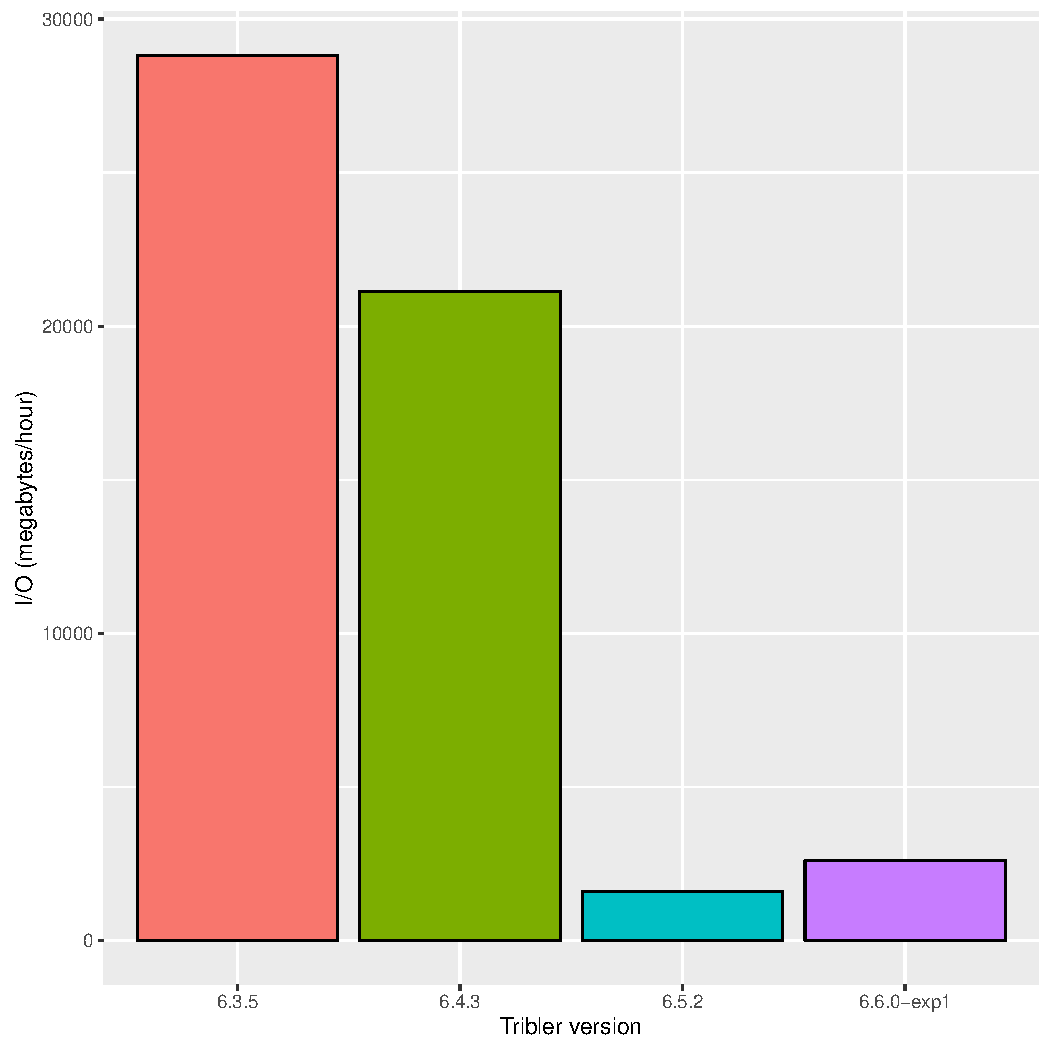
\includegraphics[width=\linewidth]{experimentation/images/io_history}
	\caption{The amount of I/O per version of Tribler.}
	\label{fig:io_history}
\end{figure} 

Each version of Tribler will run for one hour idle, using a clean state directory i.e. no prior knowledge of the network and its contents.
During the idle run, Tribler will start discovering peers and content such as channels and torrents, storing the obtained data in the database which gets flushed to disk.
Additionally, peers will start requesting data from this Tribler instance such as search and peer exchange requests, causing Tribler to read data from its database.
These read and write operations will be monitored by iotop and the amounts automatically accumulated.
After one hour, the amount of read and write I/O is noted down and Tribler is shutdown.

The results of this experiment are visible in Figure~\ref{fig:io_history}.
From this figure we observe that Tribler's I/O has been reduced significantly in version 6.5.2.
This decrease was the result of batching multiple database queries and periodically flush them to disk, an effective optimization technique also applied in other work \cite{ouyang2011beyond, lin2009database}. 
Furthermore we observe the amount of I/O is increasing again in the latest 6.6.0-exp1 release possibly due to the MultiChain feature added. 

Peculiarly, the numbers observed in this experiment are significantly higher than the numbers reported in the original ticket.
We believe there are two reasons that contribute to these numbers.
The first reason being to the 100 Mbit connection of the experiment machine, providing excellent connectability conditions. 
The second reason is the fact that this instance began with a clean state directory while running idle.
This provides ideal conditions for Tribler to spend most of its resources on discovering peers and content.

\begin{table}[]
	\centering
	\caption{The packets collected for each version by Tribler when running idle for one hour using a clean state directory.}
	\label{table:packets_collected_idle}
	\begin{tabular}{|p{7.2cm}|l|l|}
		\hline
		\textbf{Packet type}                         & \textbf{Tribler version} & \textbf{Amount}  \\ \hline
		\multirow{4}{*}{\begin{minipage}{7.2cm}Dispersy-identity: a message containing the public key of another peer for identification purposes.\end{minipage}} & 6.3.5           & 20,026  \\ \cline{2-3} 
		& 6.4.3           & 38,268  \\ \cline{2-3} 
		& 6.5.2           & 46,890  \\ \cline{2-3} 
		& 6.6.0-exp1      & 41,480  \\ \hline
		\multirow{4}{*}{\begin{minipage}{7.2cm}Dispersy-undo-own: a message that allows a member to undo his/her own messages and flags them as undone.\end{minipage}} & 6.3.5           & 40,594  \\ \cline{2-3} 
		& 6.4.3           & 45,095  \\ \cline{2-3} 
		& 6.5.2           & 47,409  \\ \cline{2-3} 
		& 6.6.0-exp1      & 44,279  \\ \hline
		\multirow{4}{*}{\begin{minipage}{7.2cm}votecast: a message indicating a vote has been given by a user on a channel, indicating it is spam or not.\end{minipage}}          & 6.3.5           & 44,990  \\ \cline{2-3} 
		& 6.4.3           & 90,339  \\ \cline{2-3} 
		& 6.5.2           & 116,557 \\ \cline{2-3} 
		& 6.6.0-exp1      & 96,509  \\ \hline
	\end{tabular}
\end{table}

To observe the cost versus the benefits, we have tracked the amount of packets Tribler managed to synchronize while running one hour idle using a clean state directory for each version.
The results are visible in Table~\ref{table:packets_collected_idle}.
From this table we conclude that while version 6.3.5 and 6.4.3 perform much more I/O, the amount of packets obtained is significantly less compared to version 6.5.2.
From these numbers we this conclude that the cost of having high I/O rates is not justified by the benefits as they perform even worse. 
Interestingly, the numbers of the latest 6.6.0-exp1 version are similar to that of 6.4.3, while we cannot explain this fully, we believe it may be caused by external network conditions or the MultiChain feature.

In conclusion, we believe that the I/O rate of Tribler does not show a correlation with the amount of packets synchronized. As the I/O rate of Tribler rises again in the latest version, possibly because of the MultiChain feature requiring additional computations, it shows the urgency of the I/O to become asynchronous and non-blocking.

\section{Detailed Database Performance Analysis}
\label{sct:db_performance_analysis}

\begin{table}[h]
	\centering
	\caption{The breakdown of Tribler's database queries when running Tribler idle for one hour using an empty state directory.}
	\label{table:query_breakdown_tribler_empty_state_dir}
	\begin{tabular}{|l|l|l|l|l|l|}
		\hline
		\textbf{Query}     & \textbf{Amount of calls} & \textbf{Total time (s)} & \textbf{Max} & \textbf{Average} & \textbf{Min} \\ \hline
		fetchall           & 91661                    & 278.319                 & 0.23420      & 0.00304          & 0.00000      \\ \hline
		execute            & 218818                   & 16.142                  & 0.21455      & 0.00007          & 0.00000      \\ \hline
		executemany        & 22558                    & 10.414                  & 0.06059      & 0.00046          & 0.00000      \\ \hline
		update             & 6647                     & 22.542                  & 0.22119      & 0.00339          & 0.00227      \\ \hline
		insert\_or\_ignore & 18511                    & 50.580                  & 0.16437      & 0.00273          & 0.00000      \\ \hline
		fetchone           & 87904                    & 273.999                 & 0.21972      & 0.00312          & 0.00196      \\ \hline
	\end{tabular}
\end{table}

\begin{table}[h]
	\centering
	\caption{The breakdown of Dispersy's database queries when running Tribler idle for one hour using an empty state directory.}
	\label{table:query_breakdown_dispersy_empty_state_dir}
	\begin{tabular}{|l|l|l|l|l|l|}
		\hline
		\textbf{Query} & \textbf{Amount of calls} & \textbf{Total time (s)} & \textbf{Max} & \textbf{Average} & \textbf{Min} \\ \hline
		commit         & 69                       & 2.758                   & 0.21891      & 0.03998          & 0.00000      \\ \hline
		execute        & 741633                   & 29.300                  & 0.14197      & 0.00004          & 0.00000      \\ \hline
		executemany    & 6781                     & 0.309                   & 0.01387      & 0.00005          & 0.00001      \\ \hline
		executescript  & 3                        & 0.000                   & 0.00001      & 0.00001          & 0.00001      \\ \hline
	\end{tabular}
\end{table}

\begin{table}[h]
	\centering
	\caption{The breakdown of Tribler's database queries when running Tribler idle for one hour using a filled state directory.}
	\label{table:query_breakdown_tribler_filled_state_dir}
	\begin{tabular}{|l|l|l|l|l|l|}
		\hline
		\textbf{Query} & \textbf{Amount of calls} & \textbf{Total time (s)} & \textbf{Max} & \textbf{Average} & \textbf{Min} \\ \hline
		fetchall   & 36815   & 318.498   & 0.46183   & 0.00865   & 0.00000   \\ \hline
		execute   & 119773   & 190.340   & 1.64548   & 0.00159   & 0.00000   \\ \hline
		executemany   & 20691   & 2.953   & 0.02570   & 0.00014   & 0.00001   \\ \hline
		update   & 8962   & 26.787   & 0.02191   & 0.00299   & 0.00221   \\ \hline
		insert\_or\_ignore   & 692   & 1.692   & 0.00483   & 0.00244   & 0.00178   \\ \hline
		fetchone   & 55090   & 171.909   & 0.96909   & 0.00312   & 0.00000   \\ \hline
	\end{tabular}
\end{table}

\begin{table}[h]
	\centering
	\caption{The breakdown of Dispersy's database queries when running Tribler idle for one hour using a filled state directory.}
	\label{table:query_breakdown_dispersy_filled_state_dir}
	\begin{tabular}{|l|l|l|l|l|l|}
		\hline
		\textbf{Query} & \textbf{Amount of calls} & \textbf{Total time (s)} & \textbf{Max} & \textbf{Average} & \textbf{Min} \\ \hline
		commit   & 68   & 24.513   & 1.65048   & 0.36048   & 0.00000   \\ \hline
		execute   & 49117   & 149.413   & 0.55947   & 0.00304   & 0.00000   \\ \hline
		executemany   & 164   & 0.004   & 0.00009   & 0.00002   & 0.00002   \\ \hline
	\end{tabular}
\end{table}

To observe the impact of each query separately, an infrastructure was created that automatically provides insight into the most expensive, most executed, and longest duration queries. 
With more than one million queries per hour, Tribler developers desperately need such a tool.
Developers can use this information to directly dive into the relevant source code and test possible improvements.
To get insight into Tribler's current query statistics, we have run two versions of Tribler for one hour using an empty state directly and a filled state directory.
A state directory is a directory where Tribler stores all configuration files, databases, information about the network and other data such as checkpoints.
The filled state directory in our experiment contains meta information on 100,000 torrents and roughly 1200 channels on which ten have been subscribed.
Such a filled state directory is quite common for regular Tribler users as they discover the network and its contents.
By subscribing to ten channels, Tribler will attempt to discover all content within these channels.

For each of the two runs, we have created breakdowns depicting the amount of queries issued on Tribler's and Dispersy's database.
The breakdowns for Tribler's database using an empty respectively filled state directory can be found in Table~\ref{table:query_breakdown_tribler_empty_state_dir} and Table~\ref{table:query_breakdown_tribler_filled_state_dir}.
In Table~\ref{table:query_breakdown_dispersy_empty_state_dir} and Table~\ref{table:query_breakdown_dispersy_filled_state_dir} we show the breakdown of Dispersy's database using an empty and filled state directory, respectively.

From these breakdowns we observe that Tribler's database I/O has an enormous impact on Tribler's performance, in contrast what was assumed by Tribler developers (see Section~\ref{sct:triblers_database_dependency}).
In the experiment with an empty state directory, Dispersy generated 32.368 seconds worth of I/O using 748,486 queries in total.
Tribler's database was queried 446,099 times, generating 651.997 seconds of I/O, a \emph{twenty fold increase} compared to Dispersy.
In total 684,365 out of 3600 seconds are spend on I/O, meaning 19\% of the time the main thread is blocked.

The situation worsens when Tribler starts filling its state directory.
Using the filled state directory, Dispersy generated 173.929 seconds worth of I/O using 49,349 queries in total.
Tribler's database was queried 242,023 times, generating 712.180 seconds of I/O.
The amount of queries is significantly lower as Dispersy now has discovered most of the network, resulting in less new peers to be added.
Additionally, less new content is discovered, reducing the amounts of operations on Tribler's database.
In general, we observe that the queries are becoming more time consuming, which can be explained by the database having more data to search through.
In total, 886,109 seconds out of 3600 seconds is spend on I/O, meaning 24.6\% of the time the main thread is blocked.

To gain insight into which functions issue the most expensive queries, we have created a breakdown of the callers for each database function.
This breakdown lists the five callers that issued queries consuming the most time.
By providing the name, file path and line number in this breakdown, developers can immediately jump to the right point in the code base, increasing the developer's productivity.
These caller breakdowns for Tribler's database when running Tribler with an empty and filled state directory are provided Table~\ref{table:caller_breakdown_tribler_empty_state_dir} and Table~\ref{table:caller_breakdown_tribler_filled_state_dir}, respectively.
Table~\ref{table:caller_breakdown_dispersy_empty_state_dir} and Table~\ref{table:caller_breakdown_dispersy_filled_state_dir} show the respective breakdowns for Dispersy's database using an empty and filled state directory.
	
\begin{table}[!h]
	\centering
	\caption{The five most expensive query issuers per database function called on Tribler's database when running Tribler idle for one hour using an empty state directory.}
	\label{table:caller_breakdown_tribler_empty_state_dir}
	\noindent\resizebox{\linewidth}{!}{
	\begin{tabular}{|c|c|c|l|}
		\hline
		\textbf{DB. function}  & \textbf{Duration (ms)} & \textbf{Caller} & \textbf{Caller location} \\ \hline
		
		\multicolumn{1}{|c|}{\multirow{5}{*}{fetchall}} & \multicolumn{1}{c|}{234} & \multicolumn{1}{c|}{getRecentAndRandomTorrents} & \multicolumn{1}{l|}{...B/SqliteCacheDBHandler.py line 1846} \\ \cline{2-4}
		\multicolumn{1}{|c|}{} & \multicolumn{1}{c|}{208}  & \multicolumn{1}{c|}{getPeerIDS}  & \multicolumn{1}{l|}{...B/SqliteCacheDBHandler.py line 101}  \\ \cline{2-4} 
		\multicolumn{1}{|c|}{} & \multicolumn{1}{c|}{205}  & \multicolumn{1}{c|}{getPeerIDS}  & \multicolumn{1}{l|}{...B/SqliteCacheDBHandler.py line 101}  \\ \cline{2-4} 
		\multicolumn{1}{|c|}{} & \multicolumn{1}{c|}{195}  & \multicolumn{1}{c|}{getPeerIDS}  & \multicolumn{1}{l|}{...B/SqliteCacheDBHandler.py line 101}  \\ \cline{2-4} 
		\multicolumn{1}{|c|}{} & \multicolumn{1}{c|}{183}  & \multicolumn{1}{c|}{getPeerIDS}  & \multicolumn{1}{l|}{...B/SqliteCacheDBHandler.py line 101}  \\ \hline 
		\multicolumn{1}{|c|}{\multirow{5}{*}{execute}} & \multicolumn{1}{c|}{214} & \multicolumn{1}{c|}{commit\_now} & \multicolumn{1}{l|}{.../CacheDB/sqlitecachedb.py line 228} \\ \cline{2-4}
		\multicolumn{1}{|c|}{} & \multicolumn{1}{c|}{198}  & \multicolumn{1}{c|}{commit\_now}  & \multicolumn{1}{l|}{.../CacheDB/sqlitecachedb.py line 228}  \\ \cline{2-4} 
		\multicolumn{1}{|c|}{} & \multicolumn{1}{c|}{193}  & \multicolumn{1}{c|}{commit\_now}  & \multicolumn{1}{l|}{.../CacheDB/sqlitecachedb.py line 228}  \\ \cline{2-4} 
		\multicolumn{1}{|c|}{} & \multicolumn{1}{c|}{182}  & \multicolumn{1}{c|}{commit\_now}  & \multicolumn{1}{l|}{.../CacheDB/sqlitecachedb.py line 228}  \\ \cline{2-4} 
		\multicolumn{1}{|c|}{} & \multicolumn{1}{c|}{165}  & \multicolumn{1}{c|}{commit\_now}  & \multicolumn{1}{l|}{.../CacheDB/sqlitecachedb.py line 228}  \\ \hline 
		\multicolumn{1}{|c|}{\multirow{5}{*}{executemany}} & \multicolumn{1}{c|}{60} & \multicolumn{1}{c|}{on\_remove\_votes\_from\_dispersy} & \multicolumn{1}{l|}{...B/SqliteCacheDBHandler.py line 1188} \\ \cline{2-4}
		\multicolumn{1}{|c|}{} & \multicolumn{1}{c|}{55}  & \multicolumn{1}{c|}{on\_remove\_votes\_from\_dispersy}  & \multicolumn{1}{l|}{...B/SqliteCacheDBHandler.py line 1188}  \\ \cline{2-4} 
		\multicolumn{1}{|c|}{} & \multicolumn{1}{c|}{52}  & \multicolumn{1}{c|}{on\_remove\_votes\_from\_dispersy}  & \multicolumn{1}{l|}{...B/SqliteCacheDBHandler.py line 1188}  \\ \cline{2-4} 
		\multicolumn{1}{|c|}{} & \multicolumn{1}{c|}{50}  & \multicolumn{1}{c|}{on\_remove\_votes\_from\_dispersy}  & \multicolumn{1}{l|}{...B/SqliteCacheDBHandler.py line 1188}  \\ \cline{2-4} 
		\multicolumn{1}{|c|}{} & \multicolumn{1}{c|}{49}  & \multicolumn{1}{c|}{on\_remove\_votes\_from\_dispersy}  & \multicolumn{1}{l|}{...B/SqliteCacheDBHandler.py line 1188}  \\ \hline 
		\multicolumn{1}{|c|}{\multirow{5}{*}{update}} & \multicolumn{1}{c|}{221} & \multicolumn{1}{c|}{addExternalTorrentNoDef} & \multicolumn{1}{l|}{...B/SqliteCacheDBHandler.py line 338} \\ \cline{2-4}
		\multicolumn{1}{|c|}{} & \multicolumn{1}{c|}{23}  & \multicolumn{1}{c|}{addExternalTorrentNoDef}  & \multicolumn{1}{l|}{...B/SqliteCacheDBHandler.py line 338}  \\ \cline{2-4} 
		\multicolumn{1}{|c|}{} & \multicolumn{1}{c|}{22}  & \multicolumn{1}{c|}{addExternalTorrentNoDef}  & \multicolumn{1}{l|}{...B/SqliteCacheDBHandler.py line 338}  \\ \cline{2-4} 
		\multicolumn{1}{|c|}{} & \multicolumn{1}{c|}{21}  & \multicolumn{1}{c|}{addExternalTorrentNoDef}  & \multicolumn{1}{l|}{...B/SqliteCacheDBHandler.py line 338}  \\ \cline{2-4} 
		\multicolumn{1}{|c|}{} & \multicolumn{1}{c|}{21}  & \multicolumn{1}{c|}{addExternalTorrentNoDef}  & \multicolumn{1}{l|}{...B/SqliteCacheDBHandler.py line 338}  \\ \hline 
		\multicolumn{1}{|c|}{\multirow{5}{*}{insert\_or\_ignore}} & \multicolumn{1}{c|}{164} & \multicolumn{1}{c|}{addOrGetPeerID} & \multicolumn{1}{l|}{...B/SqliteCacheDBHandler.py line 116} \\ \cline{2-4}
		\multicolumn{1}{|c|}{} & \multicolumn{1}{c|}{19}  & \multicolumn{1}{c|}{addOrGetPeerID}  & \multicolumn{1}{l|}{...B/SqliteCacheDBHandler.py line 116}  \\ \cline{2-4} 
		\multicolumn{1}{|c|}{} & \multicolumn{1}{c|}{18}  & \multicolumn{1}{c|}{addOrGetPeerID}  & \multicolumn{1}{l|}{...B/SqliteCacheDBHandler.py line 116}  \\ \cline{2-4} 
		\multicolumn{1}{|c|}{} & \multicolumn{1}{c|}{18}  & \multicolumn{1}{c|}{addOrGetPeerID}  & \multicolumn{1}{l|}{...B/SqliteCacheDBHandler.py line 116}  \\ \cline{2-4} 
		\multicolumn{1}{|c|}{} & \multicolumn{1}{c|}{17}  & \multicolumn{1}{c|}{addOrGetPeerID}  & \multicolumn{1}{l|}{...B/SqliteCacheDBHandler.py line 116}  \\ \hline 
		\multicolumn{1}{|c|}{\multirow{5}{*}{fetchone}} & \multicolumn{1}{c|}{219} & \multicolumn{1}{c|}{getChannelIdFromDispersyCID} & \multicolumn{1}{l|}{...B/SqliteCacheDBHandler.py line 1367} \\ \cline{2-4}
		\multicolumn{1}{|c|}{} & \multicolumn{1}{c|}{172}  & \multicolumn{1}{c|}{getOne}  & \multicolumn{1}{l|}{.../CacheDB/sqlitecachedb.py line 490}  \\ \cline{2-4} 
		\multicolumn{1}{|c|}{} & \multicolumn{1}{c|}{157}  & \multicolumn{1}{c|}{getOne}  & \multicolumn{1}{l|}{.../CacheDB/sqlitecachedb.py line 490}  \\ \cline{2-4} 
		\multicolumn{1}{|c|}{} & \multicolumn{1}{c|}{141}  & \multicolumn{1}{c|}{getChannelIdFromDispersyCID}  & \multicolumn{1}{l|}{...B/SqliteCacheDBHandler.py line 1367}  \\ \cline{2-4} 
		\multicolumn{1}{|c|}{} & \multicolumn{1}{c|}{123}  & \multicolumn{1}{c|}{getChannelIdFromDispersyCID}  & \multicolumn{1}{l|}{...B/SqliteCacheDBHandler.py line 1367}  \\ \hline 
		
	\end{tabular}}
\end{table}
		
\begin{table}[!h]
	\centering
	\caption{The five most expensive query issuers per database function called on Tribler's database when running Tribler idle for one hour using a filled state directory.}
	\label{table:caller_breakdown_tribler_filled_state_dir}
	\noindent\resizebox{\linewidth}{!}{
	\begin{tabular}{|c|c|c|l|}
		\hline
		\textbf{DB. function}  & \textbf{Duration (ms)} & \textbf{Caller} & \textbf{Caller location} \\ \hline
		\multicolumn{1}{|c|}{\multirow{5}{*}{fetchall}} & \multicolumn{1}{c|}{461} & \multicolumn{1}{c|}{\_flush\_to\_database} & \multicolumn{1}{l|}{...B/SqliteCacheDBHandler.py line 1206} \\ \cline{2-4}
		\multicolumn{1}{|c|}{} & \multicolumn{1}{c|}{437}  & \multicolumn{1}{c|}{\_flush\_to\_database}  & \multicolumn{1}{l|}{...B/SqliteCacheDBHandler.py line 1206}  \\ \cline{2-4} 
		\multicolumn{1}{|c|}{} & \multicolumn{1}{c|}{436}  & \multicolumn{1}{c|}{\_flush\_to\_database}  & \multicolumn{1}{l|}{...B/SqliteCacheDBHandler.py line 1206}  \\ \cline{2-4} 
		\multicolumn{1}{|c|}{} & \multicolumn{1}{c|}{436}  & \multicolumn{1}{c|}{\_flush\_to\_database}  & \multicolumn{1}{l|}{...B/SqliteCacheDBHandler.py line 1206}  \\ \cline{2-4} 
		\multicolumn{1}{|c|}{} & \multicolumn{1}{c|}{436}  & \multicolumn{1}{c|}{\_flush\_to\_database}  & \multicolumn{1}{l|}{...B/SqliteCacheDBHandler.py line 1206}  \\ \hline 
		\multicolumn{1}{|c|}{\multirow{5}{*}{execute}} & \multicolumn{1}{c|}{1645} & \multicolumn{1}{c|}{commit\_now} & \multicolumn{1}{l|}{.../CacheDB/sqlitecachedb.py line 228} \\ \cline{2-4}
		\multicolumn{1}{|c|}{} & \multicolumn{1}{c|}{1588}  & \multicolumn{1}{c|}{commit\_now}  & \multicolumn{1}{l|}{.../CacheDB/sqlitecachedb.py line 228}  \\ \cline{2-4} 
		\multicolumn{1}{|c|}{} & \multicolumn{1}{c|}{1465}  & \multicolumn{1}{c|}{commit\_now}  & \multicolumn{1}{l|}{.../CacheDB/sqlitecachedb.py line 228}  \\ \cline{2-4} 
		\multicolumn{1}{|c|}{} & \multicolumn{1}{c|}{1434}  & \multicolumn{1}{c|}{commit\_now}  & \multicolumn{1}{l|}{.../CacheDB/sqlitecachedb.py line 228}  \\ \cline{2-4} 
		\multicolumn{1}{|c|}{} & \multicolumn{1}{c|}{1188}  & \multicolumn{1}{c|}{commit\_now}  & \multicolumn{1}{l|}{.../CacheDB/sqlitecachedb.py line 228}  \\ \hline 
		\multicolumn{1}{|c|}{\multirow{5}{*}{executemany}} & \multicolumn{1}{c|}{25} & \multicolumn{1}{c|}{on\_remove\_votes\_from\_dispersy} & \multicolumn{1}{l|}{...B/SqliteCacheDBHandler.py line 1188} \\ \cline{2-4}
		\multicolumn{1}{|c|}{} & \multicolumn{1}{c|}{18}  & \multicolumn{1}{c|}{on\_remove\_votes\_from\_dispersy}  & \multicolumn{1}{l|}{...B/SqliteCacheDBHandler.py line 1188}  \\ \cline{2-4} 
		\multicolumn{1}{|c|}{} & \multicolumn{1}{c|}{18}  & \multicolumn{1}{c|}{on\_remove\_votes\_from\_dispersy}  & \multicolumn{1}{l|}{...B/SqliteCacheDBHandler.py line 1188}  \\ \cline{2-4} 
		\multicolumn{1}{|c|}{} & \multicolumn{1}{c|}{17}  & \multicolumn{1}{c|}{on\_remove\_votes\_from\_dispersy}  & \multicolumn{1}{l|}{...B/SqliteCacheDBHandler.py line 1188}  \\ \cline{2-4} 
		\multicolumn{1}{|c|}{} & \multicolumn{1}{c|}{15}  & \multicolumn{1}{c|}{on\_remove\_votes\_from\_dispersy}  & \multicolumn{1}{l|}{...B/SqliteCacheDBHandler.py line 1188}  \\ \hline 
		\multicolumn{1}{|c|}{\multirow{5}{*}{update}} & \multicolumn{1}{c|}{21} & \multicolumn{1}{c|}{addExternalTorrentNoDef} & \multicolumn{1}{l|}{...B/SqliteCacheDBHandler.py line 338} \\ \cline{2-4}
		\multicolumn{1}{|c|}{} & \multicolumn{1}{c|}{19}  & \multicolumn{1}{c|}{addExternalTorrentNoDef}  & \multicolumn{1}{l|}{...B/SqliteCacheDBHandler.py line 338}  \\ \cline{2-4} 
		\multicolumn{1}{|c|}{} & \multicolumn{1}{c|}{17}  & \multicolumn{1}{c|}{addExternalTorrentNoDef}  & \multicolumn{1}{l|}{...B/SqliteCacheDBHandler.py line 338}  \\ \cline{2-4} 
		\multicolumn{1}{|c|}{} & \multicolumn{1}{c|}{14}  & \multicolumn{1}{c|}{addExternalTorrentNoDef}  & \multicolumn{1}{l|}{...B/SqliteCacheDBHandler.py line 338}  \\ \cline{2-4} 
		\multicolumn{1}{|c|}{} & \multicolumn{1}{c|}{12}  & \multicolumn{1}{c|}{addExternalTorrentNoDef}  & \multicolumn{1}{l|}{...B/SqliteCacheDBHandler.py line 338}  \\ \hline 
		\multicolumn{1}{|c|}{\multirow{5}{*}{insert\_or\_ignore}} & \multicolumn{1}{c|}{4} & \multicolumn{1}{c|}{addOrGetPeerID} & \multicolumn{1}{l|}{...B/SqliteCacheDBHandler.py line 116} \\ \cline{2-4}
		\multicolumn{1}{|c|}{} & \multicolumn{1}{c|}{4}  & \multicolumn{1}{c|}{addOrGetPeerID}  & \multicolumn{1}{l|}{...B/SqliteCacheDBHandler.py line 116}  \\ \cline{2-4} 
		\multicolumn{1}{|c|}{} & \multicolumn{1}{c|}{3}  & \multicolumn{1}{c|}{addOrGetPeerID}  & \multicolumn{1}{l|}{...B/SqliteCacheDBHandler.py line 116}  \\ \cline{2-4} 
		\multicolumn{1}{|c|}{} & \multicolumn{1}{c|}{3}  & \multicolumn{1}{c|}{addOrGetPeerID}  & \multicolumn{1}{l|}{...B/SqliteCacheDBHandler.py line 116}  \\ \cline{2-4} 
		\multicolumn{1}{|c|}{} & \multicolumn{1}{c|}{3}  & \multicolumn{1}{c|}{addOrGetPeerID}  & \multicolumn{1}{l|}{...B/SqliteCacheDBHandler.py line 116}  \\ \hline 
		\multicolumn{1}{|c|}{\multirow{5}{*}{fetchone}} & \multicolumn{1}{c|}{969} & \multicolumn{1}{c|}{hasTorrents} & \multicolumn{1}{l|}{...B/SqliteCacheDBHandler.py line 1516} \\ \cline{2-4}
		\multicolumn{1}{|c|}{} & \multicolumn{1}{c|}{212}  & \multicolumn{1}{c|}{getOne}  & \multicolumn{1}{l|}{.../CacheDB/sqlitecachedb.py line 490}  \\ \cline{2-4} 
		\multicolumn{1}{|c|}{} & \multicolumn{1}{c|}{82}  & \multicolumn{1}{c|}{getOne}  & \multicolumn{1}{l|}{.../CacheDB/sqlitecachedb.py line 490}  \\ \cline{2-4} 
		\multicolumn{1}{|c|}{} & \multicolumn{1}{c|}{79}  & \multicolumn{1}{c|}{hasTorrents}  & \multicolumn{1}{l|}{...B/SqliteCacheDBHandler.py line 1516}  \\ \cline{2-4} 
		\multicolumn{1}{|c|}{} & \multicolumn{1}{c|}{73}  & \multicolumn{1}{c|}{getOne}  & \multicolumn{1}{l|}{.../CacheDB/sqlitecachedb.py line 490}  \\ \hline 
	\end{tabular}}
\end{table}
	
\begin{table}[!h]
	\centering
	\caption{The five most expensive query issuers per database function called on Dispersy's database when running Tribler idle for one hour using an empty state directory.}
	\label{table:caller_breakdown_dispersy_empty_state_dir}
	\noindent\resizebox{\linewidth}{!}{
	\begin{tabular}{|c|c|c|l|}
		\hline
		\textbf{DB. function}  & \textbf{Duration (ms)} & \textbf{Caller} & \textbf{Caller location} \\ \hline
		\multicolumn{1}{|c|}{\multirow{5}{*}{commit}} & \multicolumn{1}{c|}{218} & \multicolumn{1}{c|}{\_flush\_database} & \multicolumn{1}{l|}{...bler/dispersy/dispersy.py line 2089} \\ \cline{2-4}
		\multicolumn{1}{|c|}{} & \multicolumn{1}{c|}{204}  & \multicolumn{1}{c|}{\_flush\_database}  & \multicolumn{1}{l|}{...bler/dispersy/dispersy.py line 2089}  \\ \cline{2-4} 
		\multicolumn{1}{|c|}{} & \multicolumn{1}{c|}{198}  & \multicolumn{1}{c|}{\_flush\_database}  & \multicolumn{1}{l|}{...bler/dispersy/dispersy.py line 2089}  \\ \cline{2-4} 
		\multicolumn{1}{|c|}{} & \multicolumn{1}{c|}{186}  & \multicolumn{1}{c|}{\_flush\_database}  & \multicolumn{1}{l|}{...bler/dispersy/dispersy.py line 2089}  \\ \cline{2-4} 
		\multicolumn{1}{|c|}{} & \multicolumn{1}{c|}{169}  & \multicolumn{1}{c|}{\_flush\_database}  & \multicolumn{1}{l|}{...bler/dispersy/dispersy.py line 2089}  \\ \hline 
		\multicolumn{1}{|c|}{\multirow{5}{*}{execute}} & \multicolumn{1}{c|}{141} & \multicolumn{1}{c|}{get\_member} & \multicolumn{1}{l|}{...ler/dispersy/community.py line 1860} \\ \cline{2-4}
		\multicolumn{1}{|c|}{} & \multicolumn{1}{c|}{16}  & \multicolumn{1}{c|}{check\_undo}  & \multicolumn{1}{l|}{...ler/dispersy/community.py line 3370}  \\ \cline{2-4} 
		\multicolumn{1}{|c|}{} & \multicolumn{1}{c|}{13}  & \multicolumn{1}{c|}{initialize}  & \multicolumn{1}{l|}{...ler/dispersy/community.py line 388}  \\ \cline{2-4} 
		\multicolumn{1}{|c|}{} & \multicolumn{1}{c|}{12}  & \multicolumn{1}{c|}{get\_member}  & \multicolumn{1}{l|}{...bler/dispersy/dispersy.py line 492}  \\ \cline{2-4} 
		\multicolumn{1}{|c|}{} & \multicolumn{1}{c|}{11}  & \multicolumn{1}{c|}{get\_member}  & \multicolumn{1}{l|}{...bler/dispersy/dispersy.py line 492}  \\ \hline 
		\multicolumn{1}{|c|}{\multirow{5}{*}{executemany}} & \multicolumn{1}{c|}{13} & \multicolumn{1}{c|}{on\_undo} & \multicolumn{1}{l|}{...ler/dispersy/community.py line 3476} \\ \cline{2-4}
		\multicolumn{1}{|c|}{} & \multicolumn{1}{c|}{9}  & \multicolumn{1}{c|}{initialize}  & \multicolumn{1}{l|}{...ler/dispersy/community.py line 374}  \\ \cline{2-4} 
		\multicolumn{1}{|c|}{} & \multicolumn{1}{c|}{3}  & \multicolumn{1}{c|}{initialize}  & \multicolumn{1}{l|}{...ler/dispersy/community.py line 374}  \\ \cline{2-4} 
		\multicolumn{1}{|c|}{} & \multicolumn{1}{c|}{1}  & \multicolumn{1}{c|}{initialize}  & \multicolumn{1}{l|}{...ler/dispersy/community.py line 374}  \\ \cline{2-4} 
		\multicolumn{1}{|c|}{} & \multicolumn{1}{c|}{1}  & \multicolumn{1}{c|}{initialize}  & \multicolumn{1}{l|}{...ler/dispersy/community.py line 374}  \\ \hline 
		\multicolumn{1}{|c|}{\multirow{3}{*}{executescript}} & \multicolumn{1}{c|}{0} & \multicolumn{1}{c|}{check\_database} & \multicolumn{1}{l|}{...persy/dispersydatabase.py line 83} \\ \cline{2-4}
		\multicolumn{1}{|c|}{} & \multicolumn{1}{c|}{0}  & \multicolumn{1}{c|}{check\_database}  & \multicolumn{1}{l|}{...ty/multichain/database.py line 297}  \\ \cline{2-4} 
		\multicolumn{1}{|c|}{} & \multicolumn{1}{c|}{0}  & \multicolumn{1}{c|}{check\_database}  & \multicolumn{1}{l|}{...ty/multichain/database.py line 298}  \\ \hline 
		
	\end{tabular}}
\end{table}
	
\begin{table}[!h]
	\centering
	\caption{The five most expensive query issuers per database function called on Dispersy's database when running Tribler idle for one hour using a filled state directory.}
	\label{table:caller_breakdown_dispersy_filled_state_dir}
	\noindent\resizebox{\linewidth}{!}{
	\begin{tabular}{|c|c|c|l|}
		\hline
		\textbf{DB. function}  & \textbf{Duration (ms)} & \textbf{Caller} & \textbf{Caller location} \\ \hline
		\multicolumn{1}{|c|}{\multirow{5}{*}{commit}} & \multicolumn{1}{c|}{1650} & \multicolumn{1}{c|}{\_flush\_database} & \multicolumn{1}{l|}{...bler/dispersy/dispersy.py line 2089} \\ \cline{2-4}
		\multicolumn{1}{|c|}{} & \multicolumn{1}{c|}{1592}  & \multicolumn{1}{c|}{\_flush\_database}  & \multicolumn{1}{l|}{...bler/dispersy/dispersy.py line 2089}  \\ \cline{2-4} 
		\multicolumn{1}{|c|}{} & \multicolumn{1}{c|}{1470}  & \multicolumn{1}{c|}{\_flush\_database}  & \multicolumn{1}{l|}{...bler/dispersy/dispersy.py line 2089}  \\ \cline{2-4} 
		\multicolumn{1}{|c|}{} & \multicolumn{1}{c|}{1440}  & \multicolumn{1}{c|}{\_flush\_database}  & \multicolumn{1}{l|}{...bler/dispersy/dispersy.py line 2089}  \\ \cline{2-4} 
		\multicolumn{1}{|c|}{} & \multicolumn{1}{c|}{1194}  & \multicolumn{1}{c|}{\_flush\_database}  & \multicolumn{1}{l|}{...bler/dispersy/dispersy.py line 2089}  \\ \hline 
		\multicolumn{1}{|c|}{\multirow{5}{*}{execute}} & \multicolumn{1}{c|}{559} & \multicolumn{1}{c|}{\_select\_and\_fix} & \multicolumn{1}{l|}{...ler/dispersy/community.py line 888} \\ \cline{2-4}
		\multicolumn{1}{|c|}{} & \multicolumn{1}{c|}{548}  & \multicolumn{1}{c|}{\_select\_and\_fix}  & \multicolumn{1}{l|}{...ler/dispersy/community.py line 888}  \\ \cline{2-4} 
		\multicolumn{1}{|c|}{} & \multicolumn{1}{c|}{545}  & \multicolumn{1}{c|}{\_select\_and\_fix}  & \multicolumn{1}{l|}{...ler/dispersy/community.py line 888}  \\ \cline{2-4} 
		\multicolumn{1}{|c|}{} & \multicolumn{1}{c|}{542}  & \multicolumn{1}{c|}{\_select\_and\_fix}  & \multicolumn{1}{l|}{...ler/dispersy/community.py line 888}  \\ \cline{2-4} 
		\multicolumn{1}{|c|}{} & \multicolumn{1}{c|}{527}  & \multicolumn{1}{c|}{\_select\_and\_fix}  & \multicolumn{1}{l|}{...ler/dispersy/community.py line 888}  \\ \hline 
		\multicolumn{1}{|c|}{\multirow{5}{*}{executemany}} & \multicolumn{1}{c|}{0} & \multicolumn{1}{c|}{on\_undo} & \multicolumn{1}{l|}{...ler/dispersy/community.py line 3476} \\ \cline{2-4}
		\multicolumn{1}{|c|}{} & \multicolumn{1}{c|}{0}  & \multicolumn{1}{c|}{initialize}  & \multicolumn{1}{l|}{...ler/dispersy/community.py line 374}  \\ \cline{2-4} 
		\multicolumn{1}{|c|}{} & \multicolumn{1}{c|}{0}  & \multicolumn{1}{c|}{initialize}  & \multicolumn{1}{l|}{...ler/dispersy/community.py line 374}  \\ \cline{2-4} 
		\multicolumn{1}{|c|}{} & \multicolumn{1}{c|}{0}  & \multicolumn{1}{c|}{initialize}  & \multicolumn{1}{l|}{...ler/dispersy/community.py line 374}  \\ \cline{2-4} 
		\multicolumn{1}{|c|}{} & \multicolumn{1}{c|}{0}  & \multicolumn{1}{c|}{initialize}  & \multicolumn{1}{l|}{...ler/dispersy/community.py line 374}  \\ \hline 
	\end{tabular}}
\end{table}

In addition to creating a breakdown of the most expensive queries, we also investigated which lines contribute the most to the total amount of time spent on I/O.
By creating this breakdown we are able to identify queries that cause a lot of I/O, yet may not show up in the breakdowns above because of their low run time.
For each of the four runs mentioned above, we have computed the top five most time consuming lines and express their contribution to the total amount of time spent on I/O in percentages.
Table \ref{table:line_breakdown_tribler_empty_state_dir} and \ref{table:line_breakdown_tribler_filled_state_dir} show the top five lines which contribute the most to Tribler's database I/O time when run with an empty, respectively filled state directory.
Table \ref{table:line_breakdown_dispersy_empty_state_dir} and \ref{table:line_breakdown_dispersy_filled_state_dir} show the same breakdowns but for Dispersy's database time.
From these tables we observe that the top five lines are responsible for at least 59.9\% of all database I/O time.
Focusing on reducing these queries by applying query optimization may reduce the run times significantly \cite{jarke1984query}.

\begin{table}[!h]
	\centering
	\caption{The top five lines which contribute the most to Tribler's database I/O time using an empty state directory.}
	\label{table:line_breakdown_tribler_empty_state_dir}
	\noindent\resizebox{\linewidth}{!}{
	\begin{tabular}{|l|c|}
		\hline
		\textbf{Line} & \textbf{Contribution} \\ \hline
		/home/tribler/Documents/tribler/Tribler/Core/CacheDB/SqliteCacheDBHandler.py line 101 & 26.1\% \\ \hline
		/home/tribler/Documents/tribler/Tribler/Core/CacheDB/SqliteCacheDBHandler.py line 1367 & 24.4\% \\ \hline
		/home/tribler/Documents/tribler/Tribler/Core/CacheDB/SqliteCacheDBHandler.py line 262 & 8.0\% \\ \hline
		/home/tribler/Documents/tribler/Tribler/Core/CacheDB/SqliteCacheDBHandler.py line 116 & 7.8\% \\ \hline
		/home/tribler/Documents/tribler/Tribler/Core/CacheDB/sqlitecachedb.py line 490 & 7.0\% \\ \hline
	\end{tabular}}
\end{table}

\begin{table}[!h]
	\centering
	\caption{The top five lines which contribute the most to Tribler's database I/O time using a filled state directory.}
	\label{table:line_breakdown_tribler_filled_state_dir}
	\noindent\resizebox{\linewidth}{!}{
	\begin{tabular}{|l|c|}
		\hline
		\textbf{Line} & \textbf{Contribution} \\ \hline
		/home/tribler/Documents/tribler/Tribler/Core/CacheDB/sqlitecachedb.py line 335 & 22.9\% \\ \hline
		/home/tribler/Documents/tribler/Tribler/Core/CacheDB/SqliteCacheDBHandler.py line 1831 & 10.6\% \\ \hline
		/home/tribler/Documents/tribler/Tribler/Core/CacheDB/SqliteCacheDBHandler.py line 1820 & 10.1\% \\ \hline
		/home/tribler/Documents/tribler/Tribler/Core/CacheDB/SqliteCacheDBHandler.py line 262 & 8.3\% \\ \hline
		/home/tribler/Documents/tribler/Tribler/Core/CacheDB/sqlitecachedb.py line 490 & 8.0\% \\ \hline
	\end{tabular}}
\end{table}


\begin{table}[!h]
	\centering
	\caption{The top five lines which contribute the most to Dispersy's database I/O time using an empty state directory.}
	\label{table:line_breakdown_dispersy_empty_state_dir}
	\noindent\resizebox{\linewidth}{!}{
	\begin{tabular}{|l|c|}
		\hline
		\textbf{Line} & \textbf{Contribution} \\ \hline
		/home/tribler/Documents/tribler/Tribler/dispersy/dispersy.py line 1550 & 18.7\% \\ \hline
		/home/tribler/Documents/tribler/Tribler/dispersy/dispersy.py line 888 & 13.9\% \\ \hline
		/home/tribler/Documents/tribler/Tribler/dispersy/dispersy.py line 978 & 11.9\% \\ \hline
		/home/tribler/Documents/tribler/Tribler/dispersy/dispersy.py line 492 & 9.6\% \\ \hline
		/home/tribler/Documents/tribler/Tribler/dispersy/community.py line 3370 & 8.9\% \\ \hline
	\end{tabular}}
\end{table}

\begin{table}[!h]
\centering
\caption{The top five lines which contribute the most to Dispersy's database I/O time using a filled state directory.}
\label{table:line_breakdown_dispersy_filled_state_dir}
\noindent\resizebox{\linewidth}{!}{
\begin{tabular}{|l|c|}
	\hline
	\textbf{Line} & \textbf{Contribution} \\ \hline
	/home/tribler/Documents/tribler/Tribler/dispersy/community.py line 888 & 49.8\% \\ \hline
	/home/tribler/Documents/tribler/Tribler/dispersy/community.py line 885 & 29.7\% \\ \hline
	/home/tribler/Documents/tribler/Tribler/dispersy/dispersy.py line 2089 & 13.6\% \\ \hline
	/home/tribler/Documents/tribler/Tribler/dispersy/community.py line 914 & 5.0\% \\ \hline
	/home/tribler/Documents/tribler/Tribler/dispersy/database.py line 109 & 0.5\% \\ \hline
\end{tabular}}
\end{table}


From the results provided above we conclude what was long a hunch: Tribler is I/O bound and in desperate need of a non-blocking database I/O solution.
By creating an infrastructure which provides a breakdown of query execution statistics, we have solved the Tribler team latent need: insight into Tribler's database usage.
Using this infrastructure, developers can now focus on the queries which require optimization to adhere to the 80/20 rule: targeting the vital few, not the trivial many.

\section{Tribler's Performance Test Regression}
\label{sct:tribler_performance_regression}

To measure the performance gain of Tribler using our work, we have conducted two sets of experiments where two instances of Tribler, one with the current synchronous, blocking Dispersy implementation and one with our asynchronous, non-blocking version of Dispersy, are compared.

In the first experiment we have ran Tribler idle for one hour while querying the Twisted event loop every 100 milliseconds for delayed calls.
By doing so we can observe if certain tasks have been delayed past their set time of execution i.e. measure the latency in the system.

In the second experiment we have stress-tested Tribler's new API.
By requesting data from an endpoint at several rates per second, we can observe the response times, variance in these response times and throughput of Tribler.

\subsection{Measuring the Latency of Tribler}

\begin{table}[h]
	\centering
	\caption{Specifications of the setup used in the latency experiment.}
	\label{table:specs_hp_elitebook}
	\begin{tabular}{l|l}
		\hline
		\textbf{Component}	& \textbf{Specification} \\ \hline
		Operating System   	& Ubuntu 16.04 LTS \\
		Python version		& 2.7.12 \\
		CPU					& Intel Core i5-2410M \\ 
		HDD					& Samsung 850 EVO 250GB  \\ 
		RAM					& 8 GB DDR3 1600MHz \\
	\end{tabular}
\end{table}

\begin{figure}[!h]
	\centering
	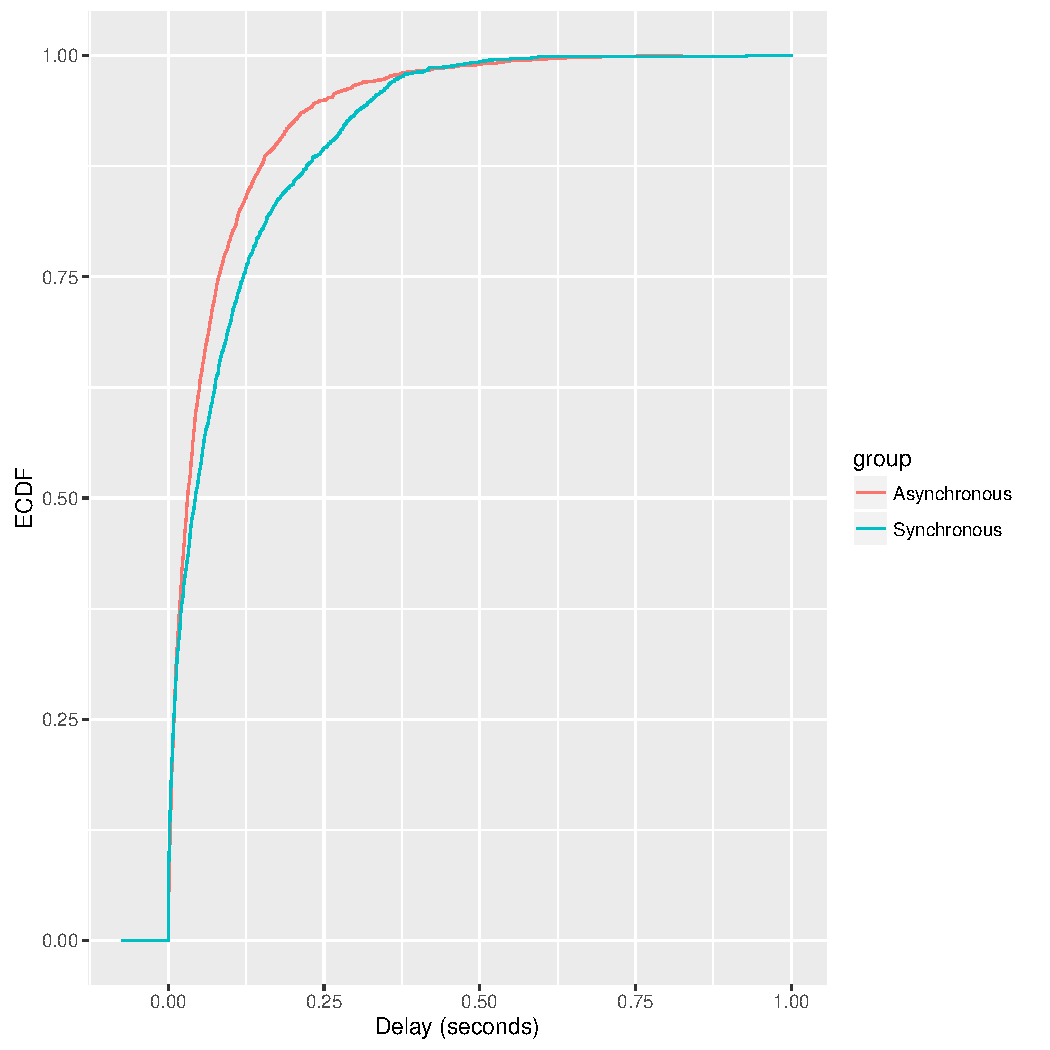
\includegraphics[width=\linewidth]{experimentation/images/ecdf_latency_idle}
	\caption{The ECDF plot showing the latency of Tribler when running idle for one hour using Dispersy with blocking, synchronous I/O and running Dispersy with non-blocking, asynchronous I/O.}
	\label{fig:ecdf_latency_idle}
\end{figure} 

In this experiment we have compared two versions of Tribler, one with Dispersy having blocking, synchronous I/O and one with Dispersy running StormDBManager and thus having non-blocking, asynchronous I/O.
This experiment was run on a machine whose specifications can be found in Table~\ref{table:specs_hp_elitebook}.
Each instance of Tribler was run one hour idle where every 100 milliseconds the event loop of Twisted was queried for delayed calls.
By observing if scheduled calls are past their set time of execution, we can measure the amount of delay or \emph{latency} in the system.
Latency occurs when the twisted reactor thread is blocked or busy with a task that takes a relative long time to complete, causing other tasks to become delayed.
Latency is therefore directly related to the responsiveness of a program.
The lower the latency, the more responsive a system is.

In theory, making functions asynchronous slices them into smaller \enquote{chunks} which can be executed interleaved, creating a more responsive system as e.g. user actions will be executed in between (background) operations.

In this experiment the hypothesis is that the latency of the asynchronous version will be lower than its synchronous counterpart.
Since Tribler is running idle it has more resources i.e. CPU time available to tend to Dispersy which is running in the background, which most likely will cause the difference to be smaller than when Tribler is experiencing additional load.
However, we believe the average may still be significant enough to prefer the asynchronous implementation.

After running the experiment, we have created an empirical cumulative distribution function (ECDF) plot of the delayed calls, visible in Figure~\ref{fig:ecdf_latency_idle}.
From this figure we observe that the asynchronous version performs better than the synchronous version.
On average, the synchronous version has a latency of 87 milliseconds, where the asynchronous version has a latency of 66 milliseconds, a reduction of 24\%.
Furthermore, the synchronous case has more outliers, some even touching the one second mark.
This confirms the hypothesis: both on average and in maxima the latency of the asynchronous version are lower.

\subsection{Measuring the Responsiveness of Tribler}
\label{sct:measuring_responsiveness_tribler}

To measure the responsiveness of Tribler while under load, we have stress tested the API of Tribler using the procedure described in Section~\ref{ssct:benchmark_3}.

In this experiment we use the filled state directory mentioned in Section~\ref{sct:db_performance_analysis}.
By querying Tribler's channel API endpoint for all discovered channels, all channels in the database will be fetched and returned.
As this is Tribler's heaviest endpoint in terms of computation, it's the best way to put Tribler under load.
In total the experiment will be run six times, querying the channel endpoint exactly 1000 times per run using 1, 2, 5, 10, 15 and 20 requests per second respectively.
By tracking the response times and the throughput (T) the API can offer, we can measure the gain in responsiveness and thus in performance of Tribler.
We expect that the asynchronous version will outperform the synchronous version significantly in both response times and throughput.

\begin{table}[!h]
	\centering
	\caption{The results of the six experiments runs with and without asynchronous, non-blocking I/O in Dispersy.}
	\label{table:responsiveness_tribler_load}
	\begin{tabular}{|c|c|c|c|c|c|c|c|}
		\hline
		Req./s              & Async. & Avg (ms) & Min & Max & Std. Dev. & T (KB/s) & Resp./s \\ \hline
		\multirow{2}{*}{1}  & \xmark      & 315 & 53  & 4774 & 615.90    & 564.19            & 0.9         \\ \cline{2-8} 
		& \cmark      & 134 & 57  & 2576 & 189.89    & 612.60            & 1.0         \\ \hline
		\multirow{2}{*}{2}  & \xmark       & 237 & 52  & 4524 & 475.31    & 1049.31           & 1.7         \\ \cline{2-8} 
		& \cmark      & 113 & 56  & 1224 & 162.62    & 1197.90           & 1.9         \\ \hline
		\multirow{2}{*}{5}  & \xmark       & 143 & 52  & 2865 & 259.64    & 2399.57           & 3.9         \\ \cline{2-8} 
		& \cmark      & 67  & 56  & 846  & 38.50     & 3058.27           & 5.0         \\ \hline
		\multirow{2}{*}{10} & \xmark       & 135 & 54  & 3338 & 259.37    & 3827.02           & 6.2         \\ \cline{2-8} 
		& \cmark      & 89  & 52  & 1138 & 92.58     & 5435.71           & 8.8         \\ \hline
		\multirow{2}{*}{15} & \xmark       & 133 & 51  & 4678 & 382.57    & 4521.46           & 7.3         \\ \cline{2-8} 
		& \cmark      & 88  & 52  & 963  & 82.23     & 6799.35           & 11.0        \\ \hline
		\multirow{2}{*}{20} & \xmark       & 109 & 51  & 3400 & 239.23    & 5599.75           & 9.1         \\ \cline{2-8} 
		& \cmark      & 74  & 52  & 1051 & 57.37     & 8264.01           & 13.4        \\ \hline
	\end{tabular}
\end{table}

\begin{figure}[!h]
	\centering
	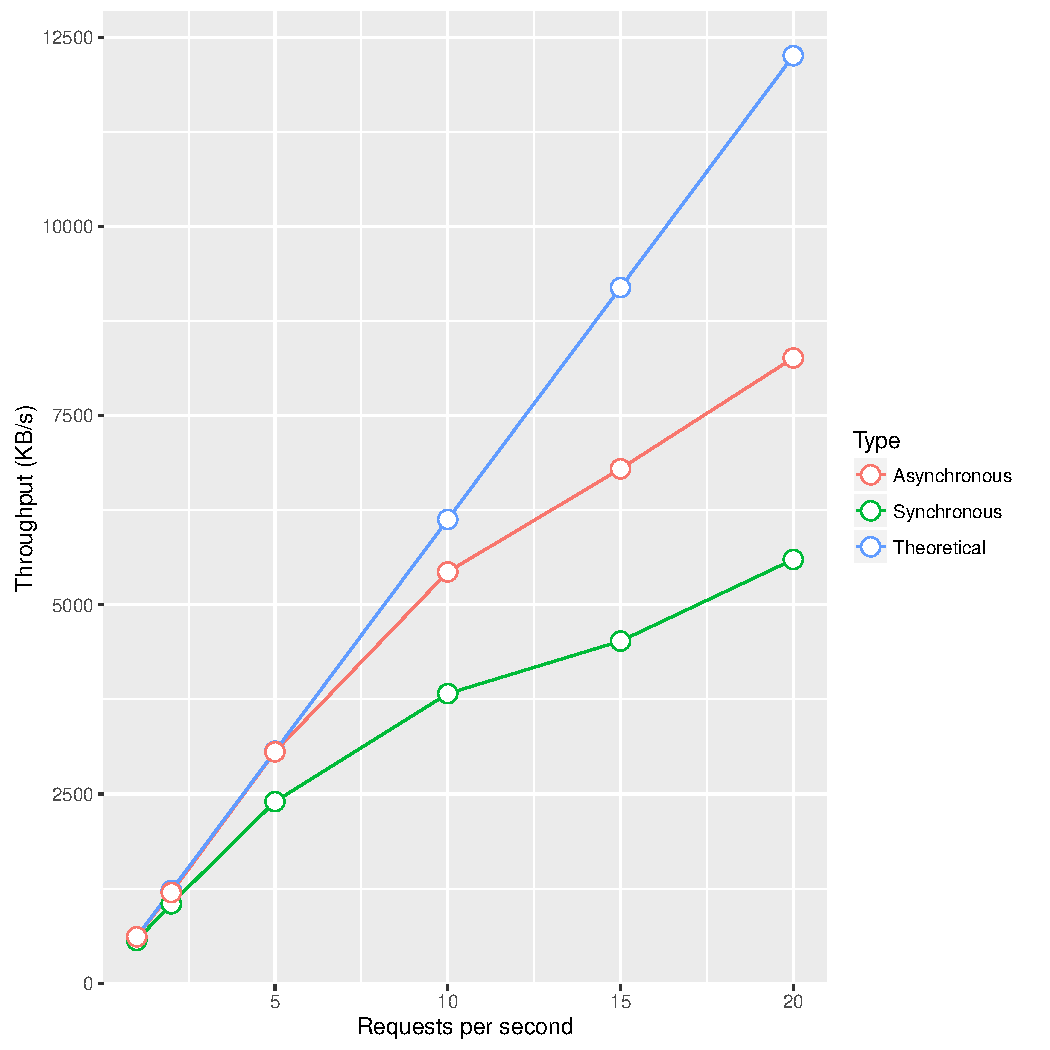
\includegraphics[width=\linewidth]{experimentation/images/throughput_requests.pdf}
	\caption{The throughput theoretically and of Tribler running Dispersy with asynchronous, non-blocking and synchronous, blocking I/O }
	\label{fig:throughput_requests}
\end{figure} 

The results of the experiment can be found in Table~\ref{table:responsiveness_tribler_load}.
From this table we observe that asynchronous version has a significant less amount of response time, both on average and in maxima.
The reduction in response times (on average) ranges between 32.1\% and 57.5\%.
As the responsiveness of a program can be directly linked to its performance (see Section~\ref{ssct:benchmark_3}), this looks very promising.
Interesting to note here is that the average response times of the synchronous version go down when the amount of requests per second goes up.
We believe this may be due to Twisted caching responses.

Another indication that the system has become more responsive is the the standard deviation.
For every run the standard deviation of the asynchronous version is significantly less than its synchronous counterpart, indicating the response times are more stable. 
This can be explained by the slicing of tasks because of asynchrony; as tasks are more interleaved, smaller tasks such as a request will be processed in between bigger tasks, yielding a higher and more stable responsivity.

A third promising statistic is the throughput.
As the response is 613 kilobytes (KB) in size, the theoretical maximum throughput will be 613, 1226, 3065, 6130, 9195 and 12260 KB/s for 1, 2, 5, 10, 15 and 20 requests per second, respectively.
If we plot the theoretical, asynchronous and the synchronous throughput we obtain Figure~\ref{fig:throughput_requests}.
As we can see the throughput of the asynchronous case lies close to the theoretical maximum until around the ten requests per second.
At this point Tribler starts to show signs of being overloaded, which is also visible in Table~\ref{table:responsiveness_tribler_load} when looking at the amount of responses received per second.

If we look at the responses per second for fifteen and twenty requests per second, we observe that the gap between requests and responses grows percentage wise.
The question that arises here is why Tribler can't provide 13.4 responses per second with fifteen requests per second as in the case with twenty.
Again we believe the answer lies in the Twisted framework.

As more tasks are scheduled on the event loop of Twisted, it will process each of them fairly where priority is given to the most delayed task.
Since there are now more requests pending, it will spend more computation power on the requests.
Even though this means that more responses per second can be provided, percentage wise the amount of replies per request drops: for fifteen requests this percentage is 73\% where for twenty requests per second this percentage is 67\%.

All in all, this experiment demonstrates that the asynchronous system has superior performance over the synchronous case, increasing the throughput by up to 150\%.

\subsection{Longtail Latencies}
\label{longtail_latencies}

Another important measurement that can be made is longtail latencies.
As Hsu explains \enquote{Longtail latencies affect members every day and improving the response times of systems even at the 99th percentile is critical to the member's experience.}, (Hsu, 2015) \cite{hsu2015who}.
Longtail latencies are latencies at high percentiles which are often orders of magnitude larger than the median latencies.
Hsu explains that longtail latencies impact users quite frequently even when the chance of one occurring is low.
If a longtail latency occurs with a probability $\rho$ and a user performs $n$ requests, the probability that a user will observe a longtail latency is 

\begin{equation}
	\label{eq:probability_high_latency}
	1 - (1 - \rho)^{n}
\end{equation}

If we take $\rho = 0.01$ and $n = 20$, the probability of a user observing a longtail latency response will be 18.2\%, a significant chance.
As the new API introduced in Tribler will be queried frequently, it is apparent that longtail latencies are also of importance to Tribler.

\begin{figure}[h]
	\begin{subfigure}[b]{.5\linewidth}
		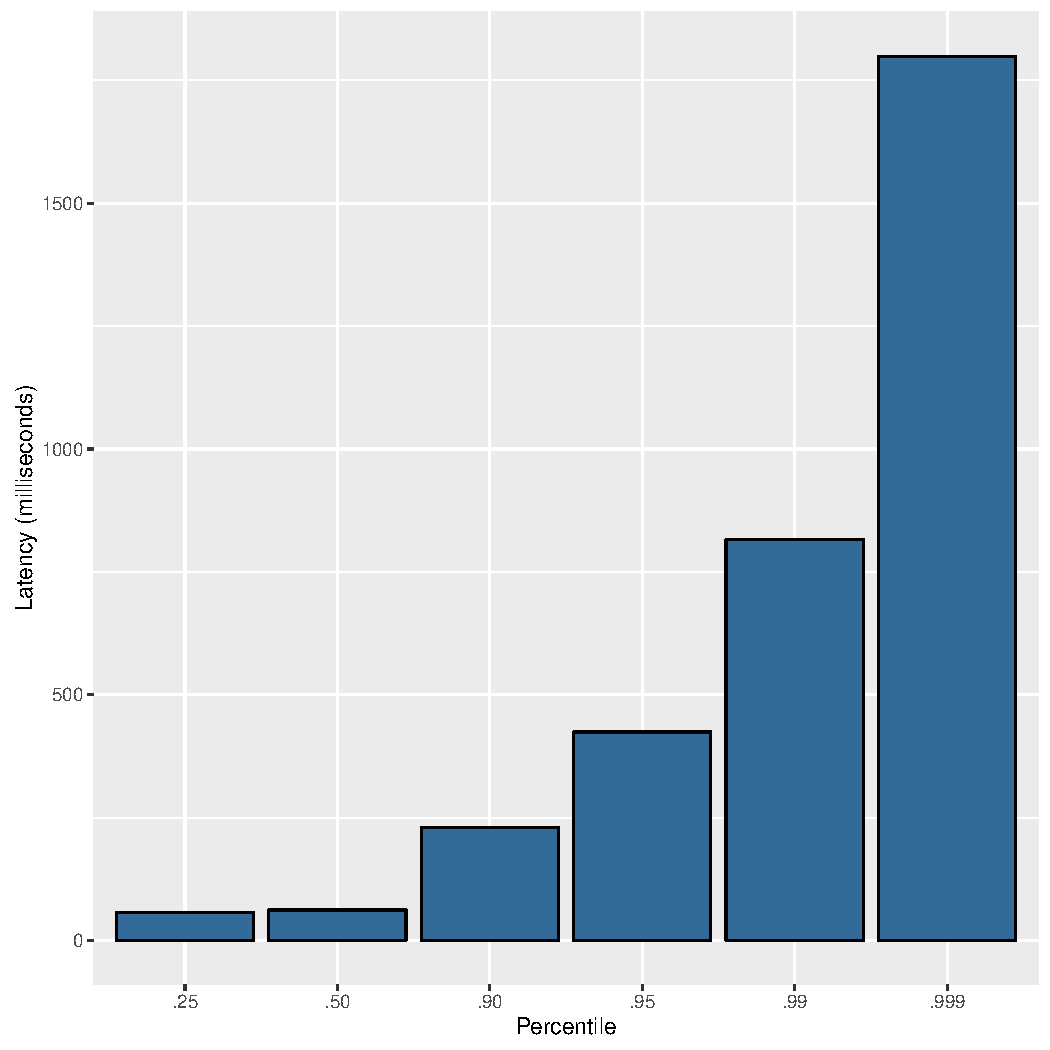
\includegraphics[width=\textwidth]{experimentation/images/response_time_percentiles_sync}
		\caption{The response times per percentile when running Dispersy with existing code.}
		\label{fig:response_times_percentiles_sync}
	\end{subfigure}
	\begin{subfigure}[b]{.5\linewidth}
		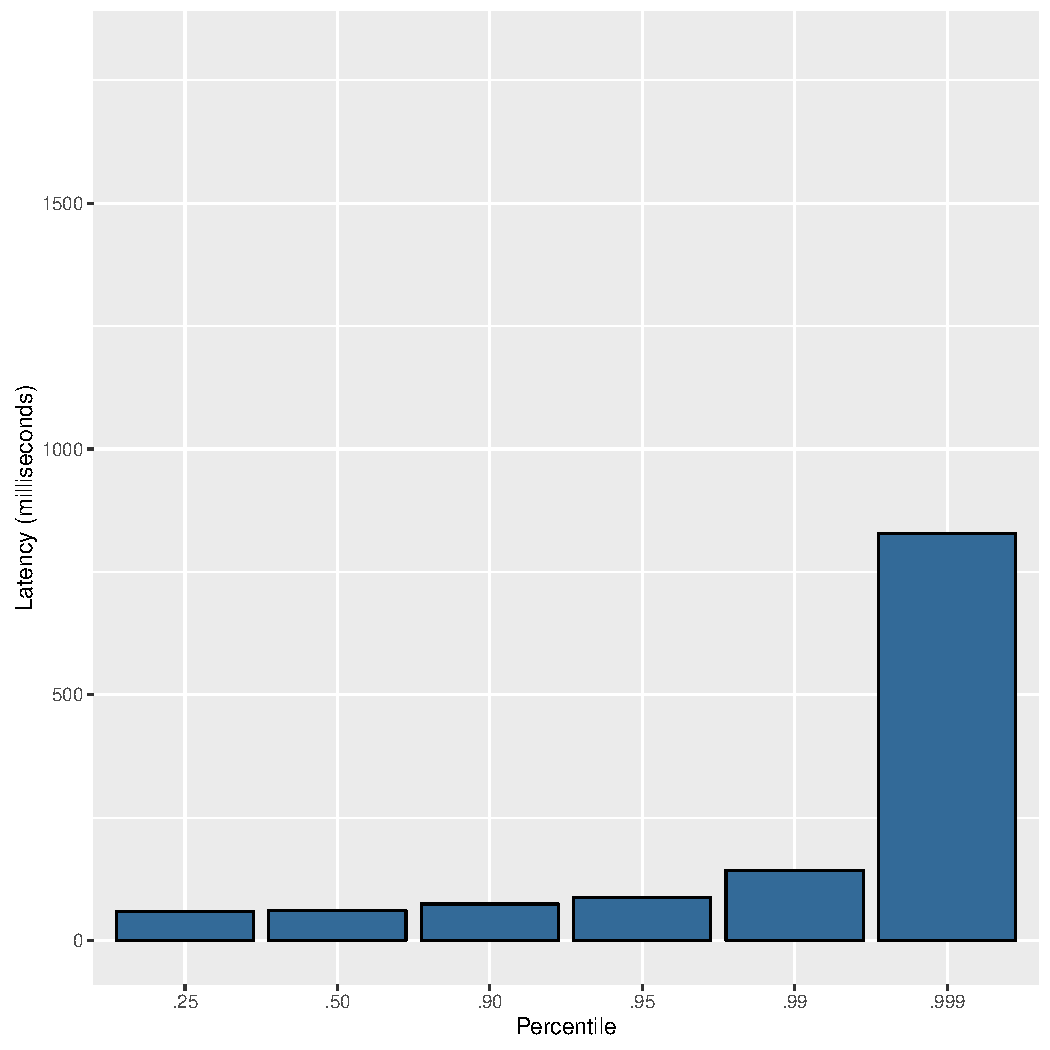
\includegraphics[width=\textwidth]{experimentation/images/response_time_percentiles_async}
		\caption{The response times per percentile when running Dispersy with our work.}
		\label{fig:response_times_percentiles_async}
	\end{subfigure}
	\caption{The response times per percentile when running Dispersy with the existing code and our work.}
	\label{fig:resposne_times_percentiles}
\end{figure}

To observe if the longtail latency problem exists in Tribler and if it has been reduced by our work, we have inspected the data generated by the experiment run conducted in Section~\ref{sct:validation_performance_regression_testing_system}.
The results are visible in Figure~\ref{fig:resposne_times_percentiles}.
From these two figures we observe that the existing code has a lot of long tail latencies, starting at the 90th percentile.
Our work starts showing long tail latencies from the 99.9th percentile, which is a huge improvement over the existing code.
However, even though we have reduced the 99.9th percentile from 1799 milliseconds in the existing code to 828 milliseconds in our work, it still indicates that work can be done to reduce this number.
As Hsu indicates, finding the root cause of these long tail percentiles can be hard and due to time constraints it is not feasible for this work to resolve.
It is therefore marked as future work.

\section{Validating the Performance Regression Testing System}
\label{sct:validation_performance_regression_testing_system}

\begin{figure}[!h]
	\centering
	\makebox[\textwidth][c]{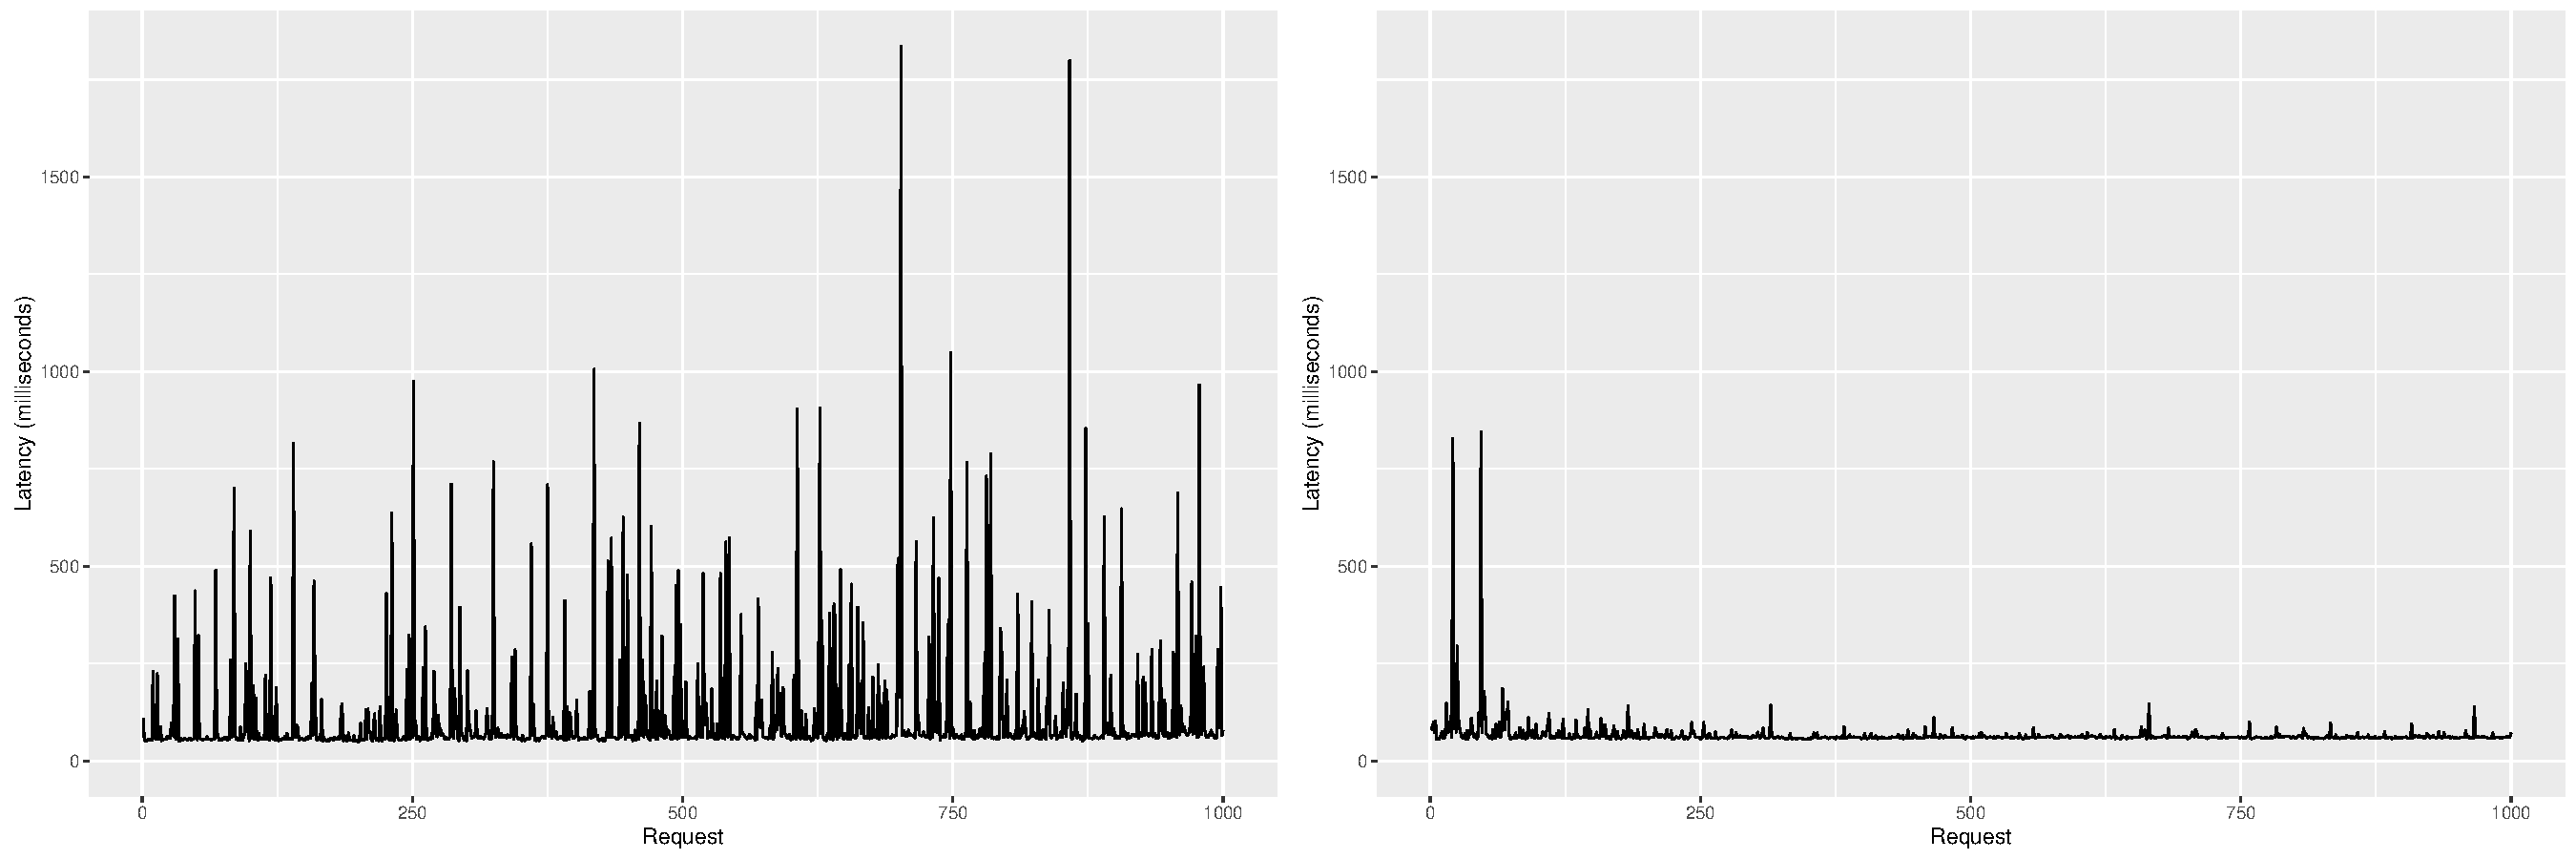
\includegraphics[width=0.9\paperwidth]{experimentation/images/response_times_comparison.pdf}}
	\caption{The comparison graph showing the response times of Tribler's API. Left: Tribler running Dispersy with synchronous, blocking I/O, right: Tribler running Dispersy with asynchronous, non-blocking I/O.}
	\label{fig:tribler_response_times_comparison}
\end{figure} 

To validate the performance regression testing system, we run the experiment described in Section~\ref{sct:measuring_responsiveness_tribler} again with five requests per second.
From the results, our regression testing system creates a side-by-side comparison graph and a table with an overview of the differences in the data obtained.

Figure~\ref{fig:tribler_response_times_comparison} shows the comparison graph generated.
From this figure, it is clear that the left hand side -- showing the existing code -- has higher response times than the right side (our work).
It is immediately clear that the proposed changes have a positive impact on the responsiveness of the API.

\begin{figure}[!h]
	\centering
	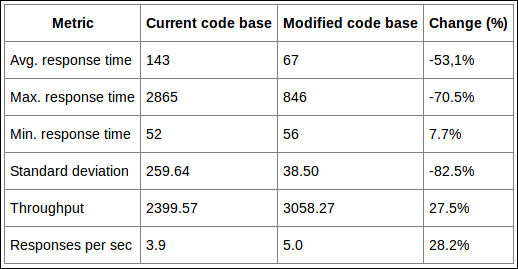
\includegraphics[width=\linewidth]{experimentation/images/table_changes}
	\caption{The generated table depicting changes between the current and modified code base.}
	\label{fig:compare_table}
\end{figure} 

To look at the data generated by the benchmark in more detail, developers can look at the table generated by the regression testing system, an example of this table is visible in Figure~\ref{fig:compare_table}.
This breakdown presents the average, minimum, maximum and standard deviation in response times as well as the throughput and amount of responses per second achieved.

From these figures we observe that the performance regression testing system provides a suitable overview for developers to get a quick overview of the changes caused by the proposed code.

\section{Summary}

From the results provided in this chapter we can conclude that Tribler is I/O bound.
By implementing a non-blocking database solution we have reduced Tribler's API response times by up to 57.5\%, improved the throughput by up to 150\% and reduced the long tail latencies considerably.
Furthermore we have finally gained insight into Tribler's database usage.
By providing a breakdown per database function and on the level of source code lines, we can now accurately pinpoint which lines are responsible for the most I/O time and which database queries might need optimization.
Finally, we have shown that our regression testing system performs well and once integrated into Tribler's development cycle, will provide detailed metrics and insights, allowing developer to pinpoint bottlenecks faster and more accurate.

Unfortunately, due to time constraints Tribler's I/O is not refactored to become asynchronous and non-blocking.
However, the foundation for Tribler's I/O to become asynchronous has been created and the insights provided are good starting points for future work.

All in all we believe we have contributed to the goal of decentralized systems such as Tribler to become as performant as centralized solutions. 
